\documentclass[12pt, twoside]{article}
\usepackage[letterpaper, margin=1in, headsep=0.5in]{geometry}
\usepackage[english]{babel}
\usepackage[utf8]{inputenc}
\usepackage{amsmath}
\usepackage{amsfonts}
\usepackage{amssymb}
\usepackage{tikz}
\usepackage{yhmath}
\usetikzlibrary{quotes, angles}

\usepackage{graphicx}
\usepackage{enumitem}
\usepackage{multicol}

\usepackage{fancyhdr}
\pagestyle{fancy}
\fancyhf{}
\renewcommand{\headrulewidth}{0pt} % disable the underline of the header

\fancyhead[RE]{\thepage}
\fancyhead[RO]{\thepage \\ Name: \hspace{3cm}}
\fancyhead[L]{BECA / Dr. Huson / 10th Grade Geometry\\* 7 May 2019}

\begin{document}
\subsubsection*{10.9 Do Now: Volume, density, trig review}
 \begin{enumerate}

   \item Find the area of a semi-circle diameter of 10. Round your answer to the  \emph{nearest tenth}.\vspace{3cm}

   \item The side $\overline{AB}$ of triangle $ABC$ is extended and an altitude to the vertex $C$ is drawn, as shown below. The triangle's height is $h=7.25$ and its base measures $AB=12.4$. Find the area of the triangle.\\[0.25cm]
   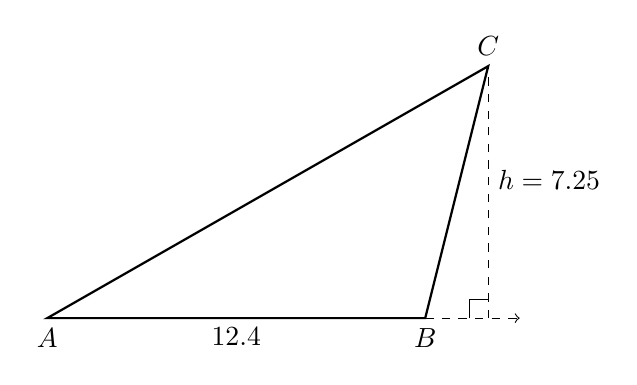
\begin{tikzpicture}[scale=0.8]
     \draw [thick]
       (0,0)node[below]{$A$}--
       (6,0)node[below]{$B$}--
       (7,4)node[above]{$C$} --cycle;
    \draw [dashed] (7,0)--(7,4);
    \draw [dashed, ->] (6,0)--(7.5,0);
    \draw (7,0)++(-0.3,0)--++(0,0.3)--+(0.3,0);
    \node at (7,2.2)[right]{$h=7.25$};
    \node at (3,0)[below]{$12.4$};
  \end{tikzpicture} \vspace{1.0cm}

  \item A crate in the shape of a rectangular prism must have a volume of 30 cubic feet. It's length is 4 feet and width 3 feet. How tall must it be? \vspace{3.0cm}

  \item Randy’s basketball is in the shape of a sphere with a maximum circumference of 29.5 inches. Determine and state the volume of the basketball, to the \emph{nearest cubic inch}.

\newpage

   \item $\triangle ABC$ is shown with $m\angle C=90^\circ$ and the lengths of the triangle's sides are $BC=8$, $AC=6$, and $AB=10$.
   \begin{multicols}{2}
         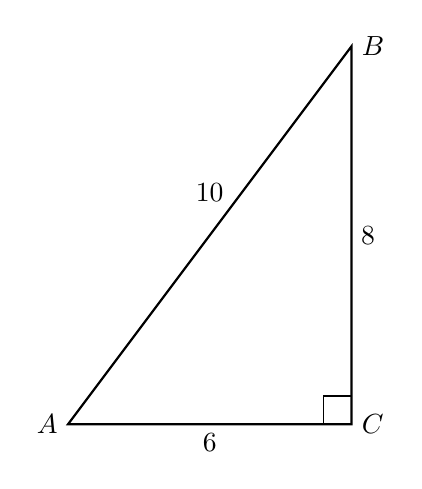
\begin{tikzpicture}[scale=0.6]
           \draw [thick]
           (0,0)node[left]{$A$}--
           (6,0)node[ right]{$C$}--
           (6,8)node[right]{$B$}--cycle;
           \draw (6,0)++(-0.6,0)--++(0,0.6)--+(0.6,0);
           \node at (3,0)[below]{$6$};
           \node at (6,4)[right]{$8$};
           \node at (3,4.5)[above]{$10$};
         \end{tikzpicture}
         \begin{enumerate}
         \item State, as a decimal, the value of $\sin A$. \vspace{0.75cm}
         \item Find the measure of $\angle A$, to the \emph{nearest degree}. \vspace{0.75cm}
         \item Find the degree measure of $\angle B$. Justify your answer.
       \end{enumerate}
     \end{multicols}
     \vspace{1.25cm}

    \item In right triangle $ABC$, hypotenuse $\overline{AB}$ has a length of 26 cm, and side $\overline{BC}$ has a length of 17.6 cm. What is the measure of angle $B$, to the \emph{nearest degree}? \vspace{3.25cm}

    \item A sailor observes the top of a lighthouse with an angle of elevation of $4^\circ$. She knows the lighthouse is 100 feet tall. Determine and state the distance $x$ between the sailor and the lighthouse, to the \emph{nearest foot}.\\[0.25cm]
    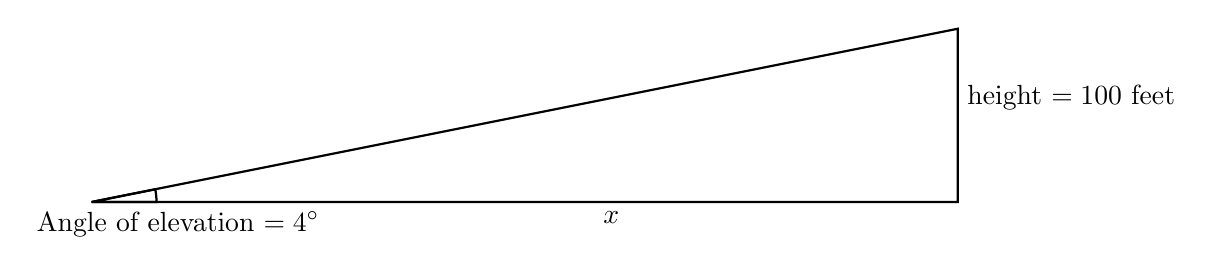
\begin{tikzpicture}[scale=1.1]
      \draw [thick] (10,0)--(0,0)--(10,2.0)--cycle;
      \draw [thick] (0,0)--(0.75,0) arc [start angle=0, end angle=11.3, radius=0.75]--cycle;
      \node at (1,0)[below]{Angle of elevation $=4^\circ$};
      \node at (10,1.2)[right]{height $=100$ feet};
      \node at (6,0)[below]{$x$};
    \end{tikzpicture} \vspace{3.25cm}

    \item If $\sin 43^\circ = \cos x$, what is the value of $x$?

  \end{enumerate}
  \newpage
  \setcounter{page}{1}
\subsubsection*{10.9 Homework: Trig review, compound volumes \& angle of elevation}
 \begin{enumerate}

  \item How many square inches are in an area one foot on each side? \vspace{2.5cm}

  \item A monument is in the shape of a pyramid with a square base whose sides measure 24 inches and whose height measures 20 feet. What is the volume of the monument, to the \emph{nearest cubic foot}? \vspace{3.5cm}

  \item A cylindrical pipe with radius $r=6$ inches has a volume of $15.7$ cubic feet. Find the length of the pipe, to the \emph{nearest foot}. \vspace{3.5cm}

  \item A weather balloon in the shape of a sphere has a volume of $7250$ cubic feet. Find the \emph{diameter} of the balloon, to the \emph{nearest foot}. \vspace{3.5cm}

\newpage

  \item A circle with a diameter of 7 in and a central angle of $60^\circ$ is drawn below.
       \begin{center}
       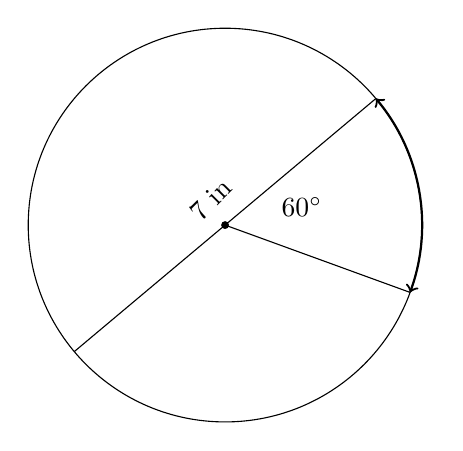
\begin{tikzpicture}[scale=.5]
         \draw (0,0) circle[radius=5];
         \draw (40:5)--(220:5);
         \draw (0,0)--(-20:5);
         \fill (0,0) circle[radius=0.1];
         \draw (13:2) node{$60^\circ$};
         \draw (120:0.75) node[rotate=45]{$7$ in};
         \draw [thick, <->] (-20:5) arc [start angle=-20, end angle=40, radius=5];
       \end{tikzpicture}
     \end{center}
  What is the length of the arc formed by the $60^\circ$ angle, to the \emph{nearest hundredth of an inch}? \vspace{2.5cm}

  What is the area of the sector formed by the $60^\circ$ angle, to the \emph{nearest hundredth of a square inch}? \vspace{2.5cm}


  \item The secants $\overline{ABC}$ and $\overline{ADE}$ intersect the circle $O$, as shown in the diagram. \\Given $m \wideparen{BD}=33^\circ$ and $m \wideparen{CE}=148^\circ$. Find the $m\angle A$.
       \begin{center}
       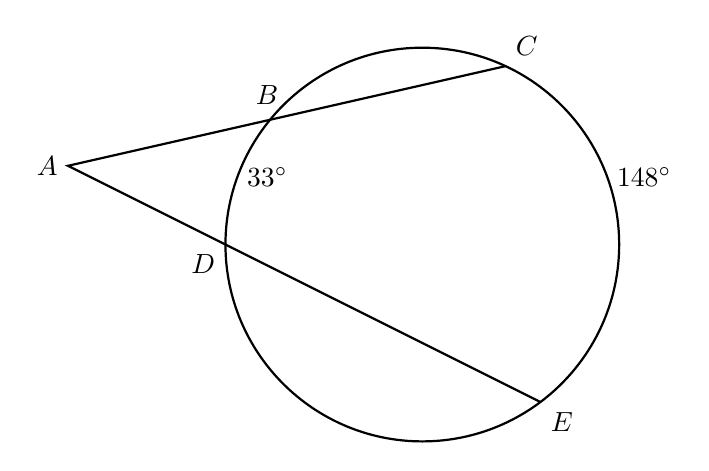
\begin{tikzpicture}[scale=.5]
         \draw [thick] (0,0) circle[radius=5];
         \draw [thick]
         (3,-4) node[below right] {$E$}--
         (-5,0) node[below left] {$D$}--
         (-9,2) node[left] {$A$}--
         (65:5) node[above right] {$C$};
         \draw (132:5.1) node[left] {$B$};
         \draw (20:5) node[right] {$148^\circ$};
         \draw (160:5) node[right] {$33^\circ$};
       \end{tikzpicture}
      \end{center}
\newpage

  \item A zipline wire is strung from a pole to the ground with an angle of elevation of $12^\circ$. If the pole is 30 feet tall, how long is the wire, to the \emph{nearest foot}.\\[0.25cm]
  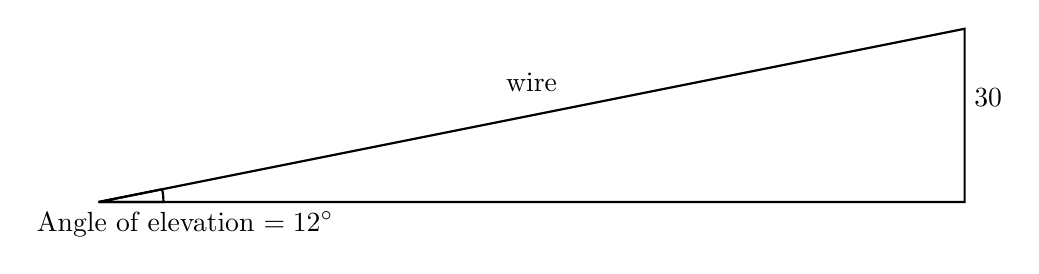
\begin{tikzpicture}[scale=1.1]
    \draw [thick] (10,0)--(0,0)--(10,2.0)--cycle;
    \draw [thick] (0,0)--(0.75,0) arc [start angle=0, end angle=11.3, radius=0.75]--cycle;
    \node at (1,0)[below]{Angle of elevation $=12^\circ$};
    \node at (10,1.2)[right]{$30$};
    \node at (5,1.6)[below]{wire};
  \end{tikzpicture} \vspace{4cm}

  \item Express each trigonometric ratio to the nearest thousandth and each angle measure to the nearest degree.
    \begin{multicols}{2}
      \begin{enumerate}
        \item $\tan 45^\circ =$ \vspace{0.5cm}
        \item $\cos 60^\circ =$
        \item $\sin^{-1} 0.450 =$ \vspace{0.5cm}
        \item $\cos^{-1} 0.950 =$
      \end{enumerate}
    \end{multicols} \vspace{0.25cm}

  \item If $\sin 65^\circ = \cos x$, what is the value of $x$? \vspace{1.5cm}

  \item $\triangle ABC$ is shown with $m\angle C=90^\circ$ and the lengths of the triangle's sides are $BC=5 \sqrt{3}$, $AC=5$, and $AB=10$.
  \begin{multicols}{2}
        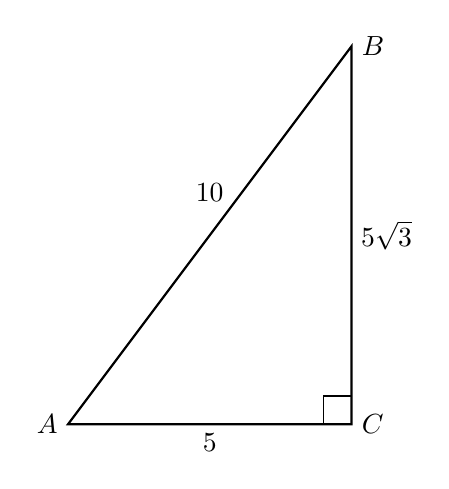
\begin{tikzpicture}[scale=0.6]
          \draw [thick]
          (0,0)node[left]{$A$}--
          (6,0)node[ right]{$C$}--
          (6,8)node[right]{$B$}--cycle;
          \draw (6,0)++(-0.6,0)--++(0,0.6)--+(0.6,0);
          \node at (3,0)[below]{$5$};
          \node at (6,4)[right]{$5 \sqrt{3}$};
          \node at (3,4.5)[above]{$10$};
        \end{tikzpicture}
        \begin{enumerate}
        \item State, as a decimal, the value of $\sin A$. \vspace{1cm}
        \item Find the measure of $\angle A$, to the \emph{nearest degree}. \vspace{1cm}
        \item Find the degree measure of $\angle B$.
      \end{enumerate}
    \end{multicols}

\newpage

  \item Given $\triangle ABC$. $\overline{AC} \cong \overline{BC}$,  $m\angle A=55$. Find $m\angle C$.\\[0.5cm]
    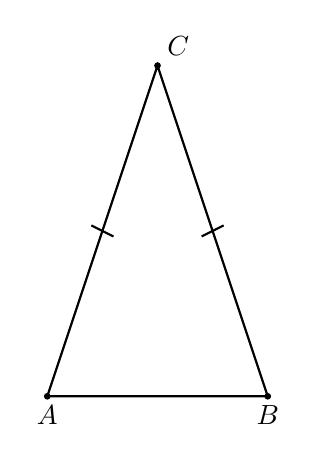
\begin{tikzpicture}[scale=0.7]
      \draw [thick](0,0)--(4,0)--(2,6)--(0,0);
      \draw [fill] (0,0) circle [radius=0.05] node[below]{$A$};
      \draw [fill] (4,0) circle [radius=0.05] node[below]{$B$};
      \draw [fill] (2,6) circle [radius=0.05] node[above right]{$C$};
      \draw [thick] (0.8,3.1)--(1.2,2.9); %tick mark
      \draw [thick] (2.8,2.9)--(3.2,3.1); %tick mark
    \end{tikzpicture}%\vspace{1cm}

  \item Given $\triangle DEF$. $\overline{DF} \cong \overline{EF}$,  $m\angle F=72$. Find $m\angle D$.\\[0.4cm]
    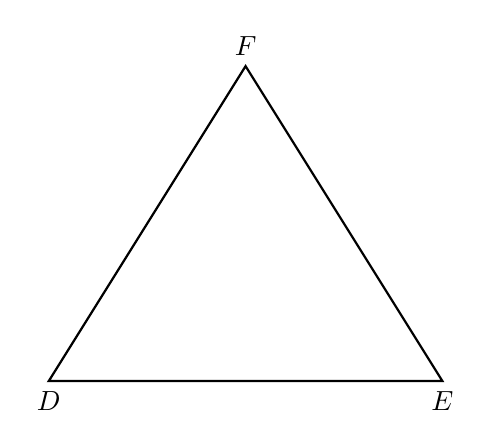
\begin{tikzpicture} %[scale=3] Isosceles, parallel marks, congruence marks
      \draw [-, thick] (0,0) node[below]{$D$}--
        (5,0) node[below]{$E$}--(2.5,4) node[above]{$F$}--cycle;
    \end{tikzpicture}\vspace{0.5cm}

  \item Given the triangle shown with congruent sides marked.  $m\angle 1=110$.
  \begin{enumerate}
    \item Find $m\angle 2$. \vspace{1.5cm}
    \item Find the measure of the vertex angle, $V$.
  \end{enumerate}
    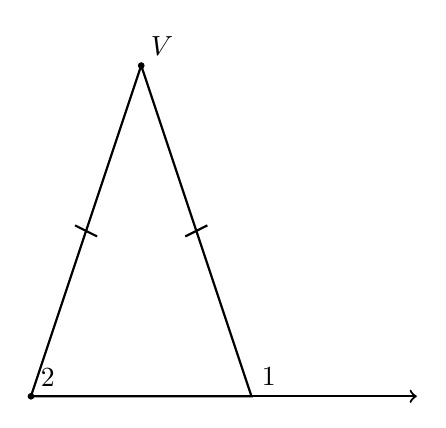
\begin{tikzpicture}[scale=0.7]
      \draw [thick](0,0)--(4,0)--(2,6)--(0,0);
      \draw [->, thick](0,0)--(4,0) node[above right]{1}--(7,0);
      \draw [fill] (0,0) circle [radius=0.05] node[above right]{$2$};
      \draw [fill] (2,6) circle [radius=0.05] node[above right]{$V$};
      \draw [thick] (0.8,3.1)--(1.2,2.9); %tick mark
      \draw [thick] (2.8,2.9)--(3.2,3.1); %tick mark
    \end{tikzpicture}


\end{enumerate}
\end{document}

\item Theresa has a rectangular pool 30 ft long, 15 ft wide, and 4 ft deep. Theresa fills her pool using city water at a rate of \$3.95 per 100 gallons of water.\\
Nancy has a circular pool with a diameter of 24 ft and a depth of 4 ft. Nancy fills her pool with a water delivery service at a rate of \$200 per 6000 gallons.\\
If Theresa and Nancy both fill their pools 6 inches from the top of the pool, determine and state who paid more to fill her pool. ($1 \mathrm{ft}^3$ water $= 1.48$ gallons)

\item As modeled in the diagram below, an access ramp starts on flat ground and ends at the beginning of the top step. Each step is 6 inches tall and 8 inches deep. \\[0.3cm]
  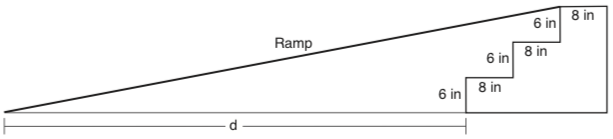
\includegraphics[width=0.8\textwidth]{ramp_Jan2019-34.png}\\
If the angle of elevation of the ramp is $4.76^\circ$, determine and state the length of the ramp, to the \emph{nearest tenth of a foot}.\\[2cm]
Determine and state, to the \emph{nearest tenth of a foot}, the horizontal distance, $d$, from the bottom of the stairs to the bottom of the ramp.
